
\documentclass[12pt]{article}
 
\usepackage[margin=1in]{geometry} 
\usepackage{amsmath,amsthm,amssymb,scrextend}
\usepackage{fancyhdr}
\pagestyle{fancy}

\usepackage{listings}
\usepackage{color}
\usepackage{geometry}
\usepackage{booktabs, multirow}

\definecolor{dkgreen}{rgb}{0,0.6,0}
\definecolor{gray}{rgb}{0.5,0.5,0.5}
\definecolor{mauve}{rgb}{0.58,0,0.82}

\lstset{frame=tb,
  language=SQL,
  aboveskip=3mm,
  belowskip=3mm,
  showstringspaces=false,
  columns=flexible,
  basicstyle={\small\ttfamily},
  numbers=none,
%   numberstyle=\tiny\color{gray},
%   keywordstyle=\color{blue},
%   commentstyle=\color{dkgreen},
%   stringstyle=\color{mauve},
  breaklines=true,
  breakatwhitespace=true,
  tabsize=3
}
\usepackage{float}
\restylefloat{table}
\newcommand{\cont}{\subseteq}
\usepackage{tikz}
\usepackage{pgfplots}
\usepackage{amsmath}
\usepackage[mathscr]{euscript}
\let\euscr\mathscr \let\mathscr\relax% just so we can load this and rsfs
\usepackage[scr]{rsfso}
\usepackage{amsthm}
\usepackage{amssymb}
\usepackage{multicol}
\usepackage[colorlinks=true, pdfstartview=FitV, linkcolor=blue,
citecolor=blue, urlcolor=blue]{hyperref}
\usepackage{graphicx}
\usepackage{subcaption}
\usepackage[utf8]{inputenc}
\usepackage[export]{adjustbox}
\usepackage{wrapfig}
\graphicspath{ {./graphs/} }

\DeclareMathOperator{\arcsec}{arcsec}
\DeclareMathOperator{\arccot}{arccot}
\DeclareMathOperator{\arccsc}{arccsc}
\newcommand{\ddx}{\frac{d}{dx}}
\newcommand{\dfdx}{\frac{df}{dx}}
\newcommand{\ddxp}[1]{\frac{d}{dx}\left( #1 \right)}
\newcommand{\dydx}{\frac{dy}{dx}}
\let\ds\displaystyle
\newcommand{\intx}[1]{\int #1 \, dx}
\newcommand{\intt}[1]{\int #1 \, dt}
\newcommand{\defint}[3]{\int_{#1}^{#2} #3 \, dx}
\newcommand{\imp}{\Rightarrow}
\newcommand{\un}{\cup}
\newcommand{\inter}{\cap}
\newcommand{\ps}{\mathscr{P}}
\newcommand{\set}[1]{\left\{ #1 \right\}}
\newtheorem*{sol}{Solution}
\newtheorem*{claim}{Claim}
\newtheorem{problem}{Problem}
\begin{document}
 
% EVERYTHING ABOVE THIS LINE IS JUST PREABLE, NO NEED TO MESS WITH IT.__________________________________________________________________________________________
%

\lhead{CS315A Assn1}
\chead{Garimella Mohan Raghu(170268)}
\rhead{\today}

\section{Queries in SQL and MongoDB}

The given table schemas were:
\begin{center}
    \texttt{ A(A1 integer, A2 string, primary-key(A1))}
    \newline
    \newline
    \texttt{ B(B1 integer, B2 integer(foreign-key = A1), B3 string, primary-key(B1))}
\end{center}

The given queries were:
\begin{itemize}
    \item {Find all tuples of A with $A1 \leq 50$.}
    \item {Find all tuples of B in sorted order of B3.}
    \item {Find average number of values per A1 by using only B table.}
    \item {Find all A2 that corresponds to B by using B2 (output the fields of B and A2).}
\end{itemize}
% \\
The queries for the above in SQL are given below:
\begin{itemize}
    \item \texttt{select * from A where A1 <= 50;}
    \item \texttt{select * from B order by B3;}
    \item \texttt{select count(*) * 1.00 / count(distinct B2)
from B;}
    \item \texttt{select B1, B2, B3, A2 from B, A where B2 = A1;}
\end{itemize}
% \\
The queries in MongoDB are given below:
\begin{itemize}
    \item \texttt{db.A.find(\{
    A1 : \{ \$lte : 50 \} 
\})}
    \item \texttt{db.B.aggregate( [ \{\$sort : \{B3:1\}\} ], \{allowDiskUse: true\})}
    \item \texttt{db.B.count() / db.B.distinct("B2").length}
\item {
    \begin{lstlisting}
db.B.aggregate ([
{ 
    $lookup : { 
        from : "A",
        localField : "B2",
        foreignField : "A1",
        as : "A" 
    } 
},
{
    $unwind : "$A"
},
{
    "$project": {
        "_id":0,
        "B1": 1,
        "B2": 1,
        "B3": 1,
        "A.A2": 1,
    }
}
])
    \end{lstlisting}
}
\end{itemize}

\section{Times Taken}

The data files assigned to me according to the last three digits of my roll number are as follows:
\begin{enumerate}
    \item { A-100.csv ,  B-100-3-4.csv }
\item { A-100.csv ,  B-100-5-2.csv }
\item { A-100.csv ,  B-100-10-1.csv }
\item { A-1000.csv ,  B-1000-5-2.csv }
\item { A-1000.csv ,  B-1000-10-1.csv }
\item { A-1000.csv ,  B-1000-50-3.csv }
\item { A-10000.csv ,  B-10000-5-1.csv }
\item { A-10000.csv ,  B-10000-50-3.csv }
\item { A-10000.csv ,  B-10000-500-4.csv }
\end{enumerate}
% \\
All the times are measured using bash \texttt{time} command at different times. 8 runs were taken and two outliers were removed.
% \begin{table}
% \centering
% \begin{tabular}{c|c|cc|cc|}
%     \toprule
%      \multirow{2}{*}{foo} & Database &
%         & \multicolumn{2}{c|}{DB1} & \multicolumn{2}{c|}{DB2}    \\
%     \cmidrule(lr){3-4} \cmidrule(lr){5-6}
%         &Time & Average  & Std.Deviation  & Average  & Std.Deviation          \\
%     \bottomrule
% %     \midrule
% % \multirow{4}{*}{SQLite} &Q1 \\ \cmidrule{2-9} &Q2 \\&Q3 \\&Q4 \\ \hline 
% %         & item 1    & item 2    & then 3    & item 4    & item 5    & item 6            \\
% %         & item 1    & item 2    & then 3    & item 4    & item 5    & item 6            \\
% %         & item 1    & item 2    & then 3    & item 4    & item 5    & item 6            \\
% %         & item 1    & item 2    & then 3    & item 4    & item 5    & item 6            \\
% %     \addlinespace
% % \multirow{4}{*}{Citation}
% %         & item 1    & item 2    & then 3    & item 4    & item 5    & item 6            \\
% %         & item 1    & item 2    & then 3    & item 4    & item 5    & item 6            \\
% %         & item 1    & item 2    & then 3    & item 4    & item 5    & item 6            \\
% %         & item 1    & item 2    & then 3    & item 4    & item 5    & item 6            \\
% %     \bottomrule
% \end{tabular}
% \caption{Example of professional table design}
% \end{table}

\begin{table}[H]
    \centering
\begin{tabular}{|c|c|c|c|c|c|}
    \hline
    \multirow{2}{*}{DBMS} & \multirow{2}{*}{Queries} & \multicolumn{2}{c|}{A-100.csv ,  B-100-3-4.csv} & \multicolumn{2}{c|}{A-100.csv ,  B-100-5-2.csv }\\
    \cline{3-6}
     & & Average & Std.Deviation & Average & Std.Deviation\\
    \hline
     \multirow{4}{*}{SQLite}& Q1 & 0.003 & 0.001 & 0.002 & 0.001 \\
\cline{2-6}
& Q2 & 0.006 & 0.001 & 0.004 & 0.002 \\
\cline{2-6}
& Q3 & 0.003 & 0.001 & 0.002 & 0.0 \\
\cline{2-6}
& Q4 & 0.006 & 0.003 & 0.003 & 0.0 \\
     \cline{2-6}
     \hline
     \multirow{4}{*}{MariaDB with Indexes} 
& Q1 & 0.005 & 0.001 & 0.005 & 0.001 \\
\cline{2-6}
& Q2 & 0.008 & 0.001 & 0.006 & 0.003 \\
\cline{2-6}
& Q3 & 0.006 & 0.001 & 0.005 & 0.0 \\
\cline{2-6}
& Q4 & 0.009 & 0.002 & 0.006 & 0.001 \\
     \cline{2-6}
    \hline
    \multirow{4}{*}{MariaDB without Indexes} 
& Q1 & 0.005 & 0.002 & 0.005 & 0.001 \\
\cline{2-6}
& Q2 & 0.008 & 0.001 & 0.007 & 0.004 \\
\cline{2-6}
& Q3 & 0.005 & 0.002 & 0.005 & 0.001 \\
\cline{2-6}
& Q4 & 0.012 & 0.004 & 0.01 & 0.002 \\
     \cline{2-6}
    \hline
    \multirow{4}{*}{MongoDB} 
& Q1 & 0.057 & 0.011 & 0.055 & 0.006 \\
\cline{2-6}
& Q2 & 0.081 & 0.01 & 0.077 & 0.008 \\
\cline{2-6}
& Q3 & 0.052 & 0.01 & 0.049 & 0.002 \\
\cline{2-6}
& Q4 & 0.115 & 0.024 & 0.105 & 0.01 \\

     \cline{2-6}
    \hline
\end{tabular}

    \caption{Times for DB 1,2 in seconds}
    \label{tab:my_label}
\end{table}

\begin{table}[H]
    \centering
\begin{tabular}{|c|c|c|c|c|c|}
    \hline
    \multirow{2}{*}{DBMS} & \multirow{2}{*}{Queries} & \multicolumn{2}{c|}{A-100.csv , B-100-10-1.csv} & \multicolumn{2}{c|}{A-1000.csv , B-1000-5-2.csv}\\
    \cline{3-6}
     & & Average & Std.Deviation & Average & Std.Deviation\\
    \hline
     \multirow{4}{*}{SQLite} & Q1 & 0.003 & 0.001 & 0.003 & 0.0 \\
\cline{2-6}
& Q2 & 0.004 & 0.003 & 0.006 & 0.002 \\
\cline{2-6}
& Q3 & 0.003 & 0.001 & 0.003 & 0.0 \\
\cline{2-6}
& Q4 & 0.003 & 0.0 & 0.005 & 0.001 \\
     \cline{2-6}
     \hline
     \multirow{4}{*}{MariaDB with Indexes} 
& Q1 & 0.005 & 0.001 & 0.005 & 0.0 \\
\cline{2-6}
& Q2 & 0.008 & 0.005 & 0.013 & 0.003 \\
\cline{2-6}
& Q3 & 0.006 & 0.001 & 0.006 & 0.0 \\
\cline{2-6}
& Q4 & 0.006 & 0.001 & 0.01 & 0.002 \\
     \cline{2-6}
    \hline
    \multirow{4}{*}{MariaDB without Indexes} 
& Q1 & 0.005 & 0.0 & 0.005 & 0.0 \\
\cline{2-6}
& Q2 & 0.007 & 0.004 & 0.013 & 0.003 \\
\cline{2-6}
& Q3 & 0.006 & 0.001 & 0.006 & 0.0 \\
\cline{2-6}
& Q4 & 0.01 & 0.002 & 0.272 & 0.017 \\
     \cline{2-6}
    \hline
    \multirow{4}{*}{MongoDB}
& Q1 & 0.054 & 0.003 & 0.054 & 0.007 \\
\cline{2-6}
& Q2 & 0.092 & 0.009 & 0.312 & 0.026 \\
\cline{2-6}
& Q3 & 0.055 & 0.01 & 0.053 & 0.01 \\
\cline{2-6}
& Q4 & 0.129 & 0.008 & 1.437 & 0.044 \\
     \cline{2-6}
    \hline
\end{tabular}

    \caption{Times for DB 3,4 in seconds}
    \label{tab:my_label}
\end{table}

\newpage

\begin{table}[H]
    \centering
\begin{tabular}{|c|c|c|c|c|c|}
    \hline
    \multirow{2}{*}{DBMS} & \multirow{2}{*}{Queries} & \multicolumn{2}{c|}{A-1000.csv , B-1000-10-1.csv} & \multicolumn{2}{c|}{A-1000.csv , B-1000-50-3.csv}\\
    \cline{3-6}
     & & Average & Std.Deviation & Average & Std.Deviation\\
    \hline
     \multirow{4}{*}{SQLite}& Q1 & 0.002 & 0.0 & 0.002 & 0.001 \\
\cline{2-6}
& Q2 & 0.008 & 0.0 & 0.027 & 0.001 \\
\cline{2-6}
& Q3 & 0.003 & 0.0 & 0.006 & 0.0 \\
\cline{2-6}
& Q4 & 0.008 & 0.002 & 0.02 & 0.001 \\
     \cline{2-6}
     \hline
     \multirow{4}{*}{MariaDB with Indexes} & Q1 & 0.005 & 0.001 & 0.005 & 0.0 \\
\cline{2-6}
& Q2 & 0.017 & 0.001 & 0.062 & 0.001 \\
\cline{2-6}
& Q3 & 0.006 & 0.0 & 0.012 & 0.0 \\
\cline{2-6}
& Q4 & 0.014 & 0.001 & 0.034 & 0.002 \\

     \cline{2-6}
    \hline
    \multirow{4}{*}{MariaDB without Indexes} 
& Q1 & 0.005 & 0.001 & 0.005 & 0.0 \\
\cline{2-6}
& Q2 & 0.018 & 0.0 & 0.078 & 0.013 \\
\cline{2-6}
& Q3 & 0.007 & 0.001 & 0.015 & 0.001 \\
\cline{2-6}
& Q4 & 0.46 & 0.011 & 2.029 & 0.043 \\
     \cline{2-6}
    \hline
    \multirow{4}{*}{MongoDB} 
& Q1 & 0.066 & 0.021 & 0.081 & 0.022 \\
\cline{2-6}
& Q2 & 0.483 & 0.011 & 1.957 & 0.114 \\
\cline{2-6}
& Q3 & 0.064 & 0.021 & 0.105 & 0.019 \\
\cline{2-6}
& Q4 & 2.513 & 0.079 & 11.246 & 0.186 \\

     \cline{2-6}
    \hline
\end{tabular}

    \caption{Times for DB 5,6 in seconds}
    \label{tab:my_label}
\end{table}

\begin{table}[H]
    \centering
\begin{tabular}{|c|c|c|c|c|c|}
    \hline
    \multirow{2}{*}{DBMS} & \multirow{2}{*}{Queries} & \multicolumn{2}{c|}{A-10000.csv, B-10000-5-1.csv} & \multicolumn{2}{c|}{A-10000.csv, B-10000-50-3.csv}\\
    \cline{3-6}
     & & Average & Std.Deviation & Average & Std.Deviation\\
    \hline
     \multirow{4}{*}{SQLite} & Q1 & 0.003 & 0.0 & 0.002 & 0.0 \\
\cline{2-6}
& Q2 & 0.036 & 0.004 & 0.257 & 0.015 \\
\cline{2-6}
& Q3 & 0.009 & 0.0 & 0.036 & 0.001 \\
\cline{2-6}
& Q4 & 0.027 & 0.001 & 0.181 & 0.013 \\
     \cline{2-6}
     \hline
     \multirow{4}{*}{MariaDB with Indexes} 
& Q1 & 0.005 & 0.0 & 0.005 & 0.0 \\
\cline{2-6}
& Q2 & 0.078 & 0.003 & 0.69 & 0.05 \\
\cline{2-6}
& Q3 & 0.017 & 0.001 & 0.084 & 0.001 \\
\cline{2-6}
& Q4 & 0.048 & 0.002 & 0.29 & 0.013 \\
     \cline{2-6}
    \hline
    \multirow{4}{*}{MariaDB without Indexes} 
& Q1 & 0.008 & 0.001 & 0.008 & 0.001 \\
\cline{2-6}
& Q2 & 0.087 & 0.006 & 0.754 & 0.098 \\
\cline{2-6}
& Q3 & 0.022 & 0.004 & 0.106 & 0.002 \\
\cline{2-6}
& Q4 & 25.942 & 0.806 & 198.116 & 9.495 \\
     \cline{2-6}
    \hline
    \multirow{4}{*}{MongoDB} 
& Q1 & 0.096 & 0.025 & 0.073 & 0.022 \\
\cline{2-6}
& Q2 & 2.597 & 0.319 & 18.209 & 1.097 \\
\cline{2-6}
& Q3 & 0.107 & 0.016 & 0.206 & 0.022 \\
\cline{2-6}
& Q4 & 109.824 & 3.635 & 822.083 & 31.48 \\

     \cline{2-6}
    \hline
\end{tabular}

    \caption{Times for DB 7,8 in seconds}
    \label{tab:my_label}
\end{table}

\newpage

\begin{table}[H]
    \centering
\begin{tabular}{|c|c|c|c|}
    \hline
    \multirow{2}{*}{DBMS} & \multirow{2}{*}{Queries} & \multicolumn{2}{c|}{A-10000.csv , B-10000-500-4.csv}\\
    \cline{3-4}
     & & Average & Std.Deviation \\
    \hline
     \multirow{4}{*}{SQLite} & Q1 & 0.003 & 0.001 \\
\cline{2-4}
& Q2 & 2.695 & 0.107 \\
\cline{2-4}
& Q3 & 0.311 & 0.014 \\
\cline{2-4}
& Q4 & 1.765 & 0.082 \\
\cline{2-4}

     \hline
     \multirow{4}{*}{MariaDB with Indexes}
& Q1 & 0.005 & 0.0 \\
\cline{2-4}
& Q2 & 11.712 & 2.56 \\
\cline{2-4}
& Q3 & 0.852 & 0.022 \\
\cline{2-4}
& Q4 & 13.219 & 0.983 \\
\cline{2-4}
    \hline
    \multirow{4}{*}{MariaDB without Indexes} 
& Q1 & 0.008 & 0.001 \\
\cline{2-4}
& Q2 & 12.31 & 1.296 \\
\cline{2-4}
& Q3 & 1.064 & 0.035 \\
\cline{2-4}
& Q4 & 1908.729 & 48.294 \\
\cline{2-4}
    \hline
    \multirow{4}{*}{MongoDB} 
& Q1 & 0.102 & 0.015 \\
\cline{2-4}
& Q2 & 171.175 & 9.505 \\
\cline{2-4}
& Q3 & 1.238 & 0.032 \\
\cline{2-4}
& Q4 & 7920.63 & 233.188 \\
\cline{2-4}

    \hline
\end{tabular}

    \caption{Times for DB 9 in seconds}
    \label{tab:my_label}
\end{table}

\newpage

\section{Graphs}

Some of the graphs below may be difficult to interpret due to wide range of values for Time. For more detailed graphs refer to the directory \texttt{170268/graphs/extra}.

\subsection{DBMS vs Time Taken for each Query}

\begin{figure}[H]
  \centering
  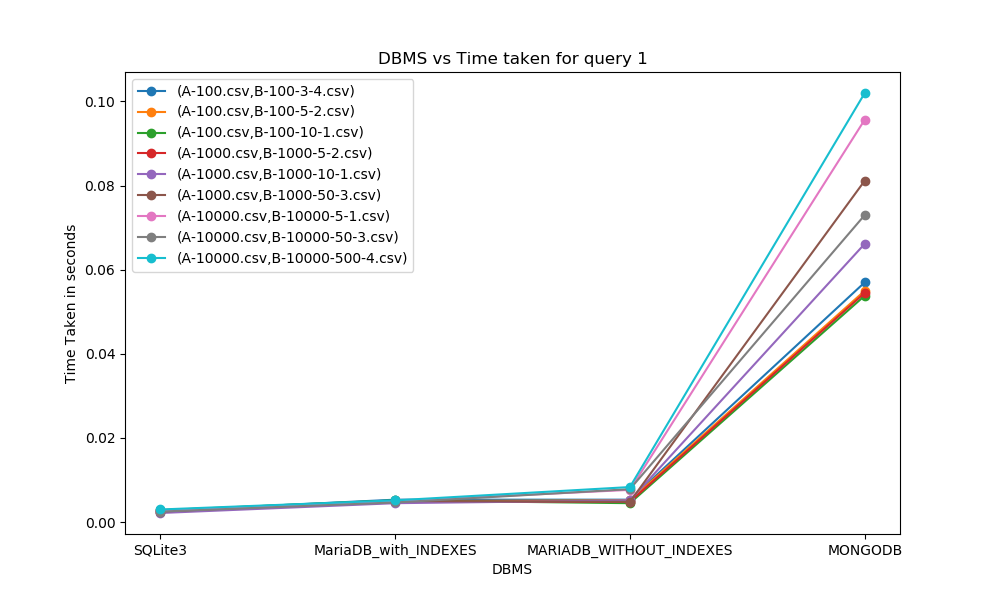
\includegraphics[width=.95\linewidth]{dbms_time/1.png}
\end{figure}

\begin{figure}[H]
  \centering
  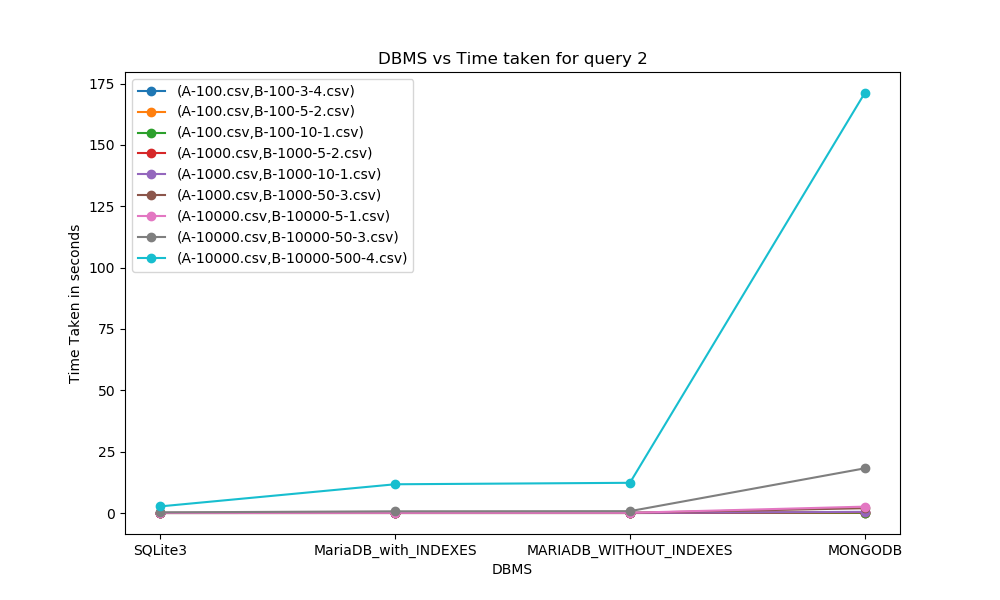
\includegraphics[width=.95\linewidth]{dbms_time/2.png}
\end{figure}

\begin{figure}[H]
  \centering
  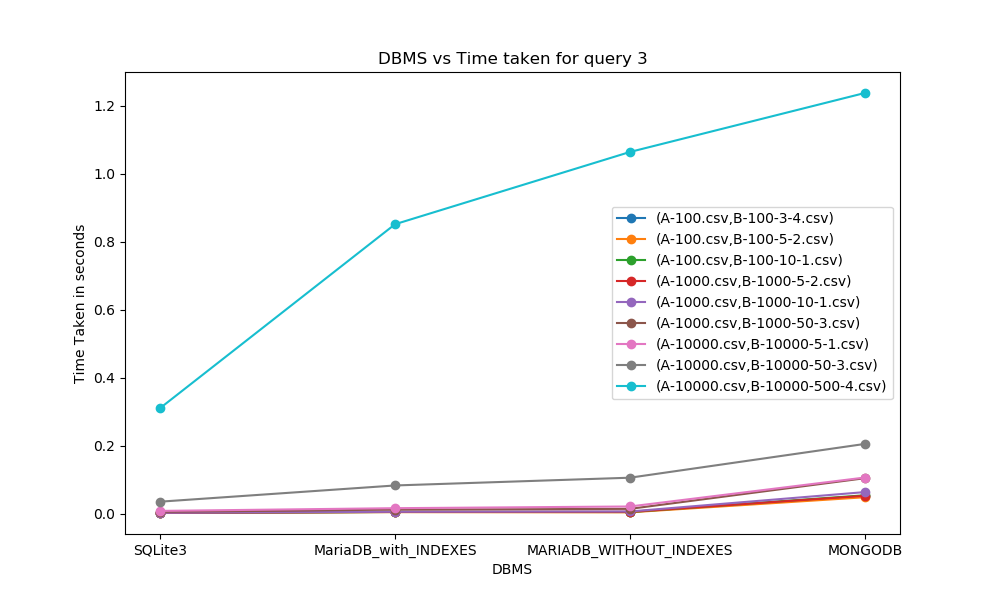
\includegraphics[width=.95\linewidth]{dbms_time/3.png}
\end{figure}

\begin{figure}[H]
  \centering
  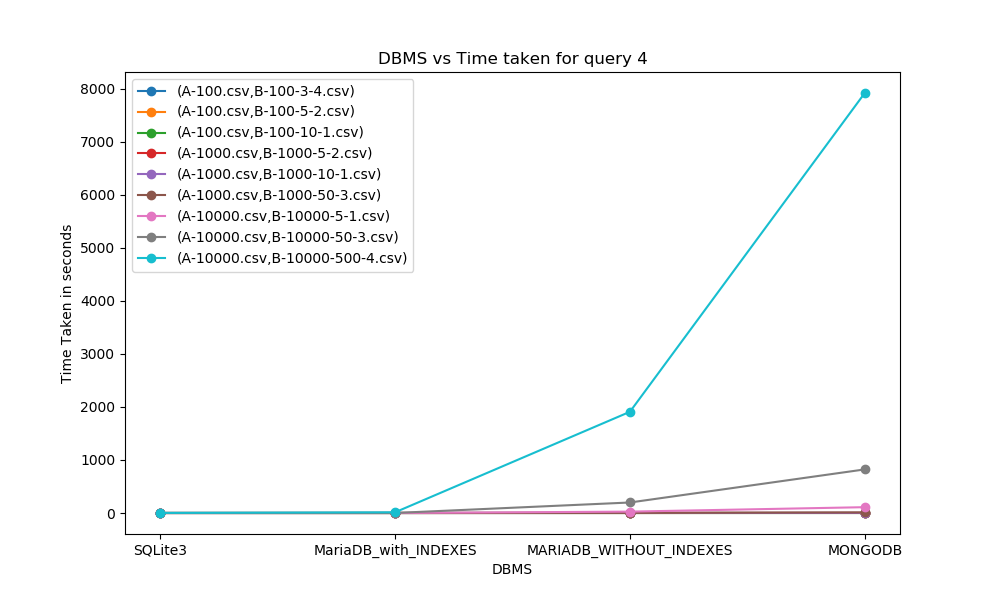
\includegraphics[width=.95\linewidth]{dbms_time/4.png}
\end{figure}


\subsection{Query vs Time Taken for each Database}

\begin{figure}[H]
  \centering
  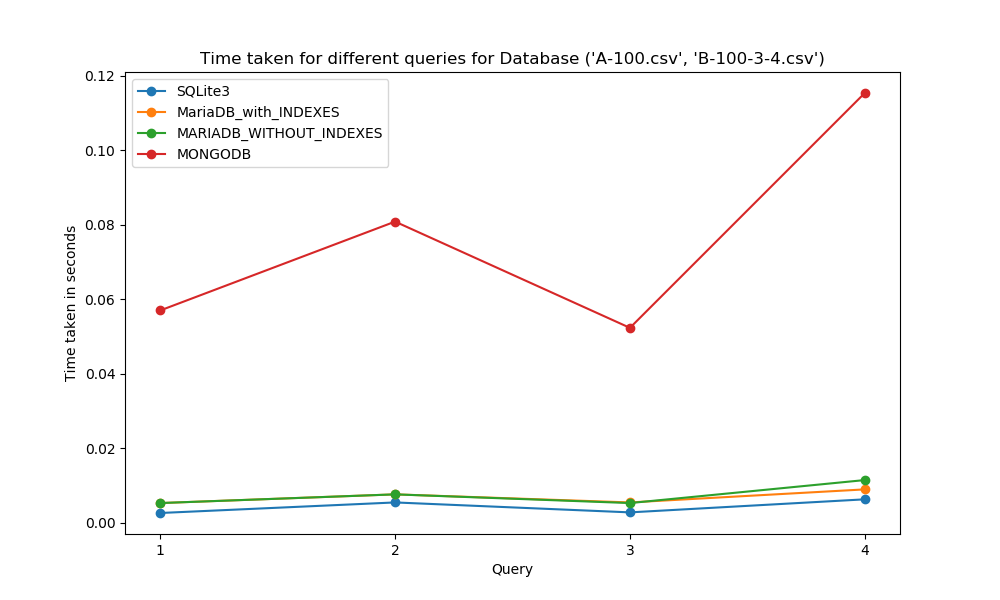
\includegraphics[width=.95\linewidth]{db_qry_time/1.png}
\end{figure}

\begin{figure}[H]
  \centering
  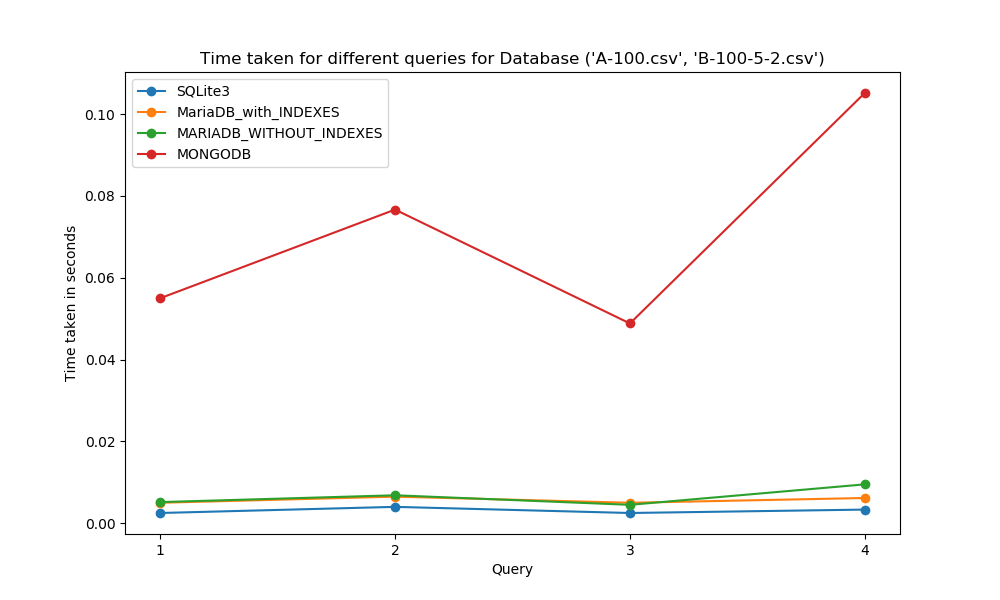
\includegraphics[width=.95\linewidth]{db_qry_time/2.png}
\end{figure}

\begin{figure}[H]
  \centering
  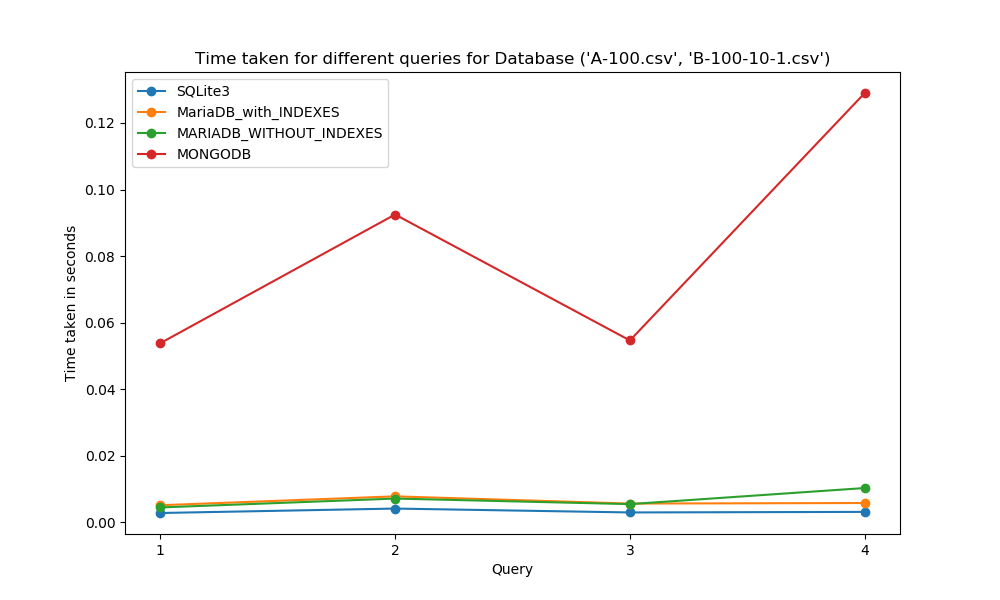
\includegraphics[width=.95\linewidth]{db_qry_time/3.png}
\end{figure}

\begin{figure}[H]
  \centering
  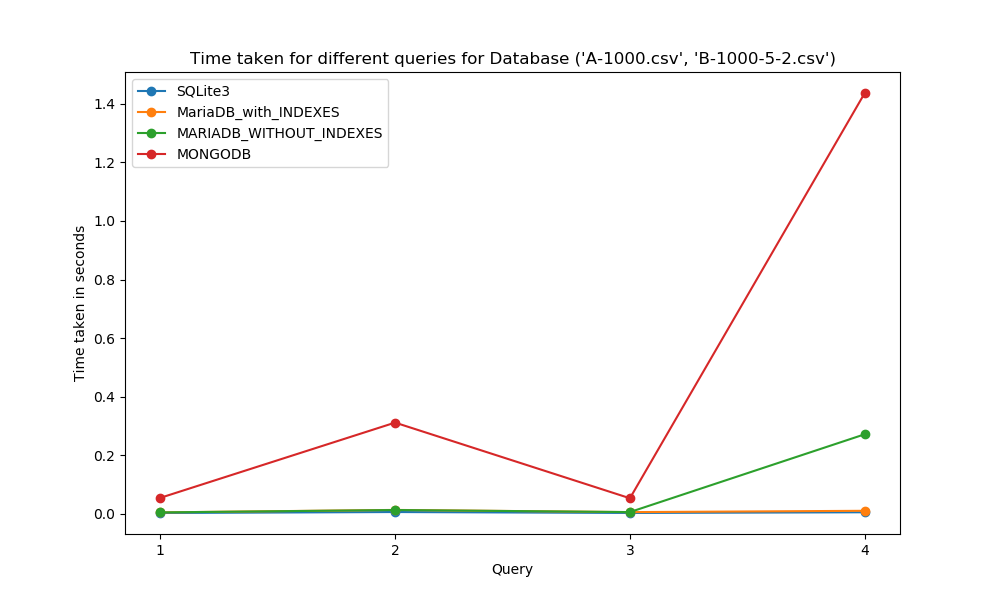
\includegraphics[width=.95\linewidth]{db_qry_time/4.png}
\end{figure}
\begin{figure}[H]
  \centering
  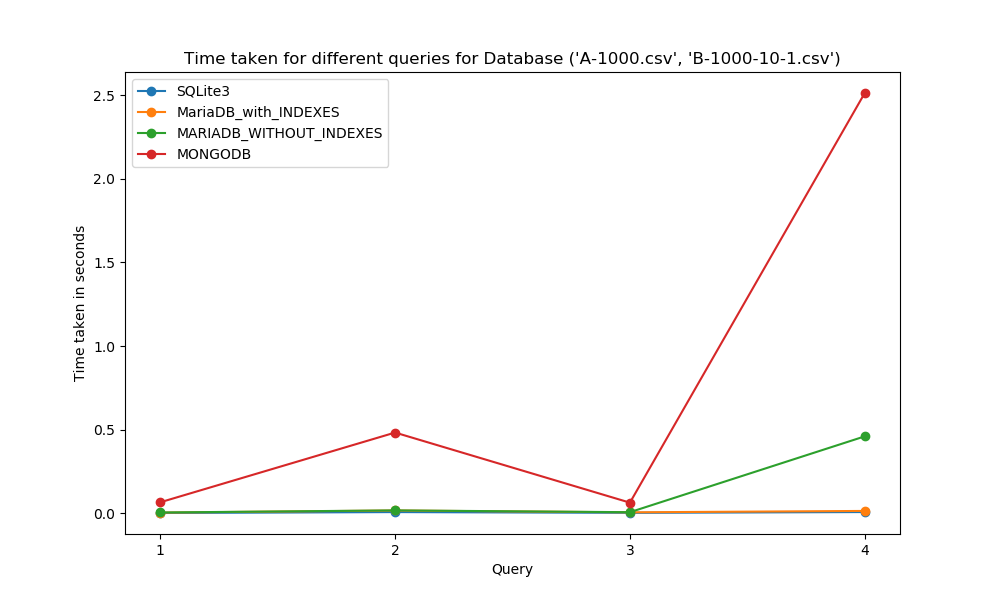
\includegraphics[width=.95\linewidth]{db_qry_time/5.png}
\end{figure}

\begin{figure}[H]
  \centering
  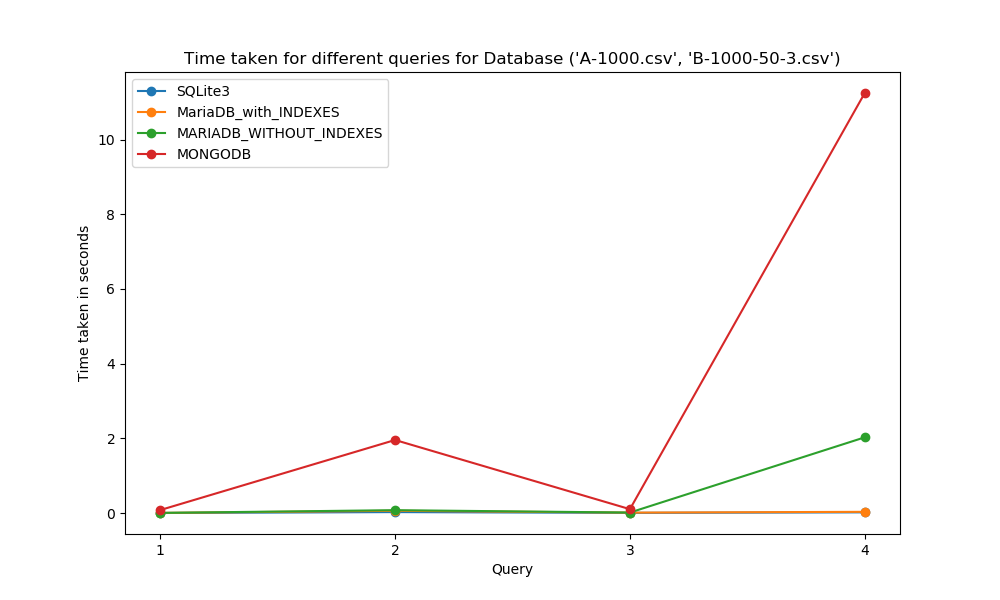
\includegraphics[width=.95\linewidth]{db_qry_time/6.png}
\end{figure}

\begin{figure}[H]
  \centering
  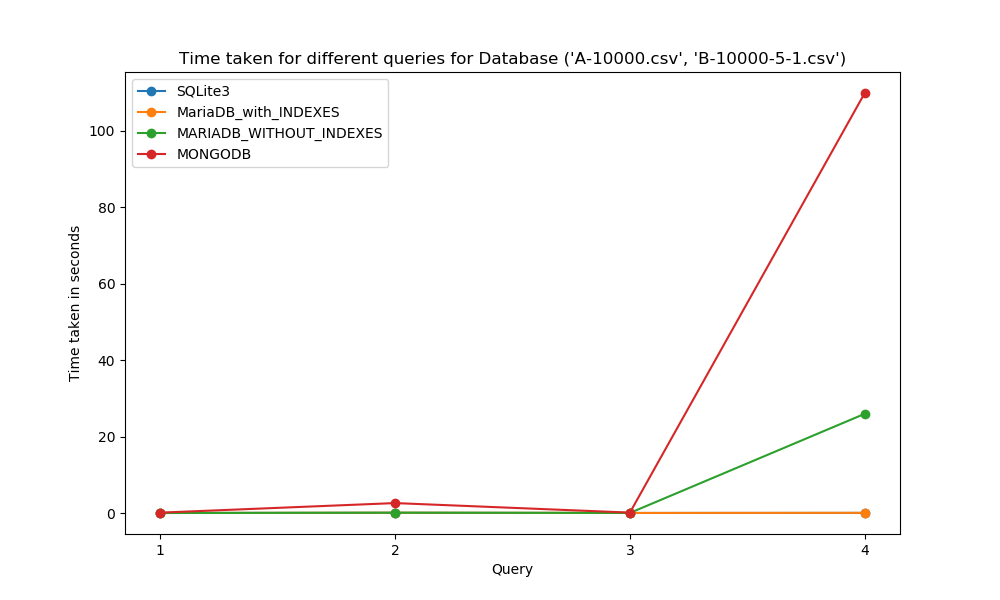
\includegraphics[width=.95\linewidth]{db_qry_time/7.png}
\end{figure}

\begin{figure}[H]
  \centering
  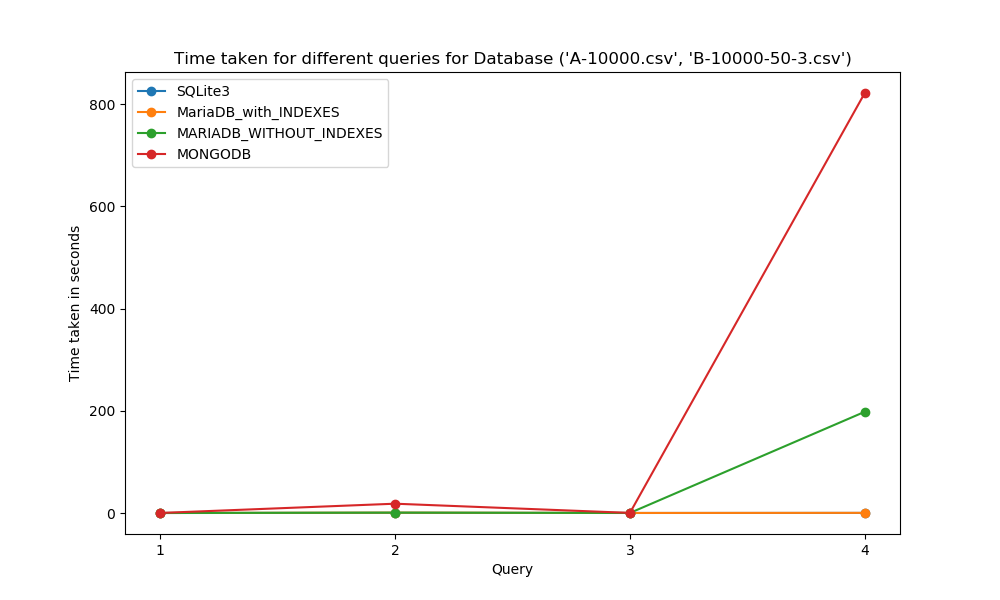
\includegraphics[width=.95\linewidth]{db_qry_time/8.png}
\end{figure}

\begin{figure}[H]
  \centering
  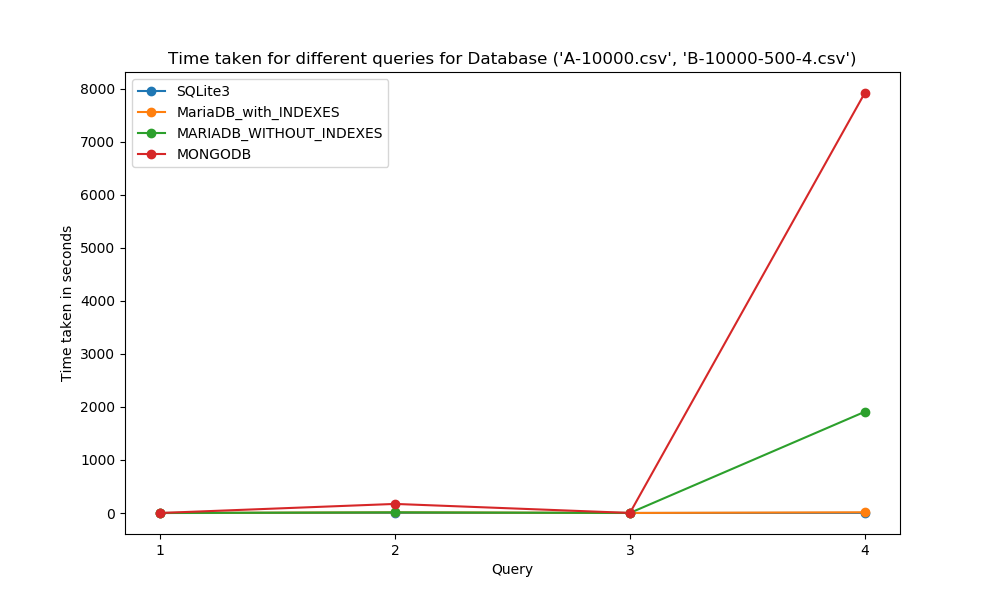
\includegraphics[width=.95\linewidth]{db_qry_time/9.png}
\end{figure}

\subsection{Database Size vs Time Taken for each Query}
\begin{figure}[H]
  \centering
  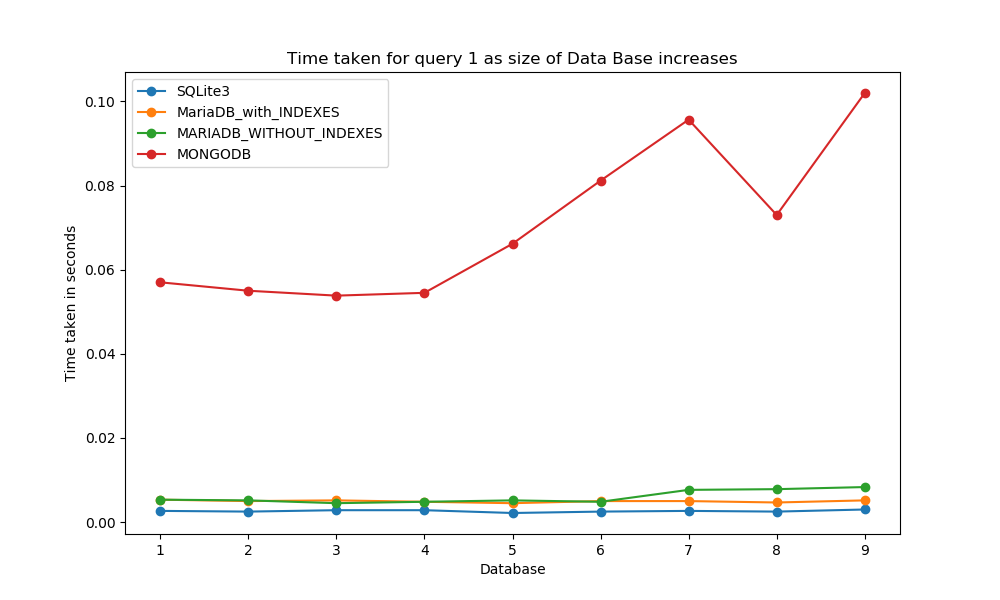
\includegraphics[width=.95\linewidth]{db_size_time/1.png}
\end{figure}

\begin{figure}[H]
  \centering
  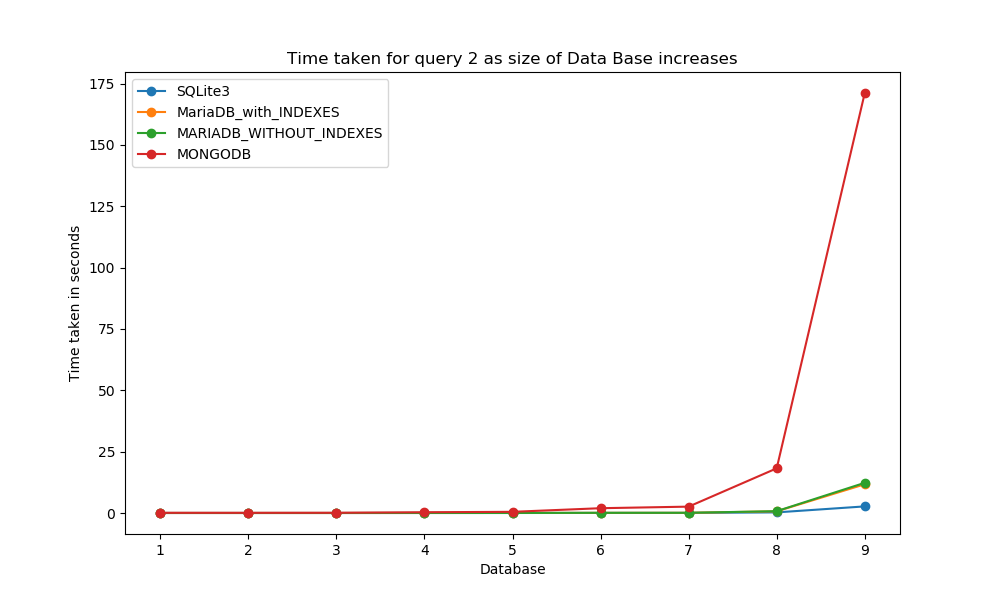
\includegraphics[width=.95\linewidth]{db_size_time/2.png}
\end{figure}

\begin{figure}[H]
  \centering
  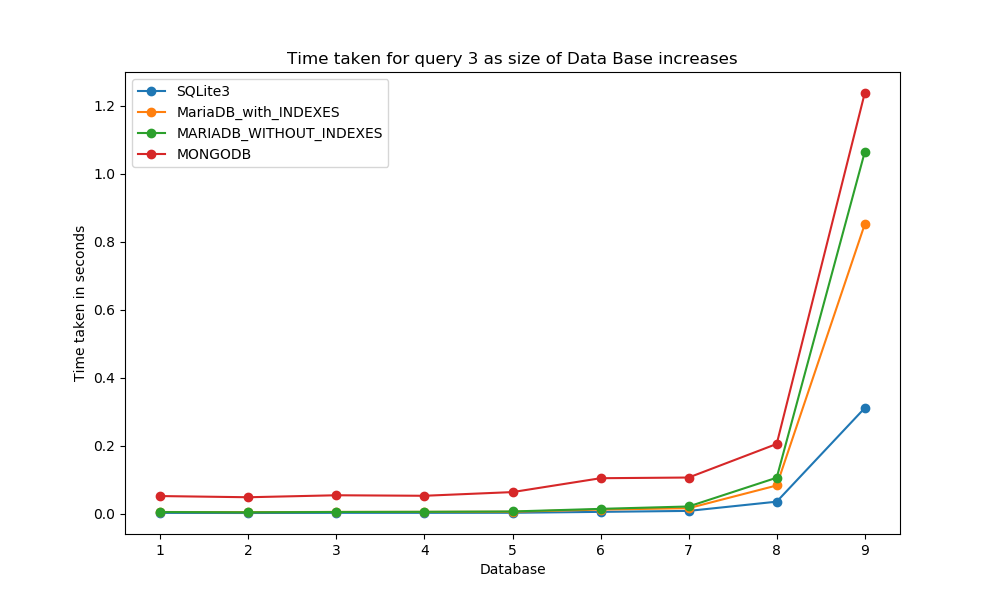
\includegraphics[width=.95\linewidth]{db_size_time/3.png}
\end{figure}

\begin{figure}[H]
  \centering
  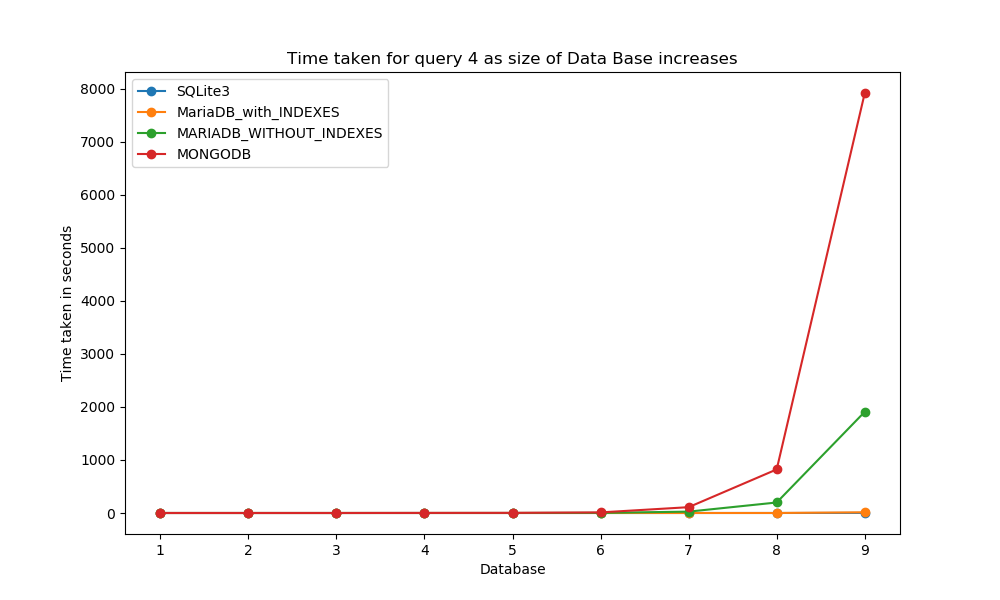
\includegraphics[width=.95\linewidth]{db_size_time/4.png}
\end{figure}

\section{Conclusions}

Specifications of the Machine on which the above measurements are as follows:
\begin{center}
\texttt{OS: Ubuntu 20.04 focal} \\
\texttt{RAM: 16GB} \\
\texttt{CPU: Intel Core i7-8750H @ 12x 4.1GHz} \\
\texttt{Disk: 1TB HDD/256 GB SSD} \\
\texttt{SQLite Version : 3.31.1} \\
\texttt{MariaDB Version : 10.3.25-MariaDB-0ubuntu0.20.04.1}\\
\texttt{MongoDB Version : 4.4.4}\\
\end{center}


\begin{itemize}
   \item \textbf{Scaling of Queries: }As size of Database increases, the time taken also increases for all the 
   Database management systems. The difference in time is more significant for Queries 2 and 4 compared to others, it may be since query 2 involves comparison 
   of strings and Q4 is a computationally heavy join operation which takes time proportional to product of entries in A and B. Also among the
   database management systems, the difference is more significant in MariaDB without Indexes and MongoDB compared to others.  
This is because of absence of indexes and non-relational nature of MongoDB.

\item \textbf{Comparison among Queries: }The order of Times taken for the queries is $Q4 > Q2 > Q3 > Q1$. The trend is self explanatory, Q1 involves a simple select operation on A and also A has fewer entries
compared to B hence it is significantly faster than other queries, Q2 and Q3 are similar except that Q2 involves comparison of Strings(B3), while Q3 involves comparison of integers(B2) so Q3 is
faster than Q2. Q4 is slower than all other queries since it involves join of two tables.

\item \textbf{Comparison among DBMS: } The order of Times taken for all the four queries was found to be
MongoDB $>$ MariaDB\_without\_Indexes $>$ MariaDB\_with\_indexes $>$ SQLite. Since MongoDB is a no sql database and others are
relational databases, the queries run slower in MongoDB compared to others. As expected, MariaDB with indexes runs faster than
MariaDB without indexes.SQLite and MariaDB with Indexes take almost same time which is expected because SQLite builds indexes on primary and foreign keys by default. An interesting observation is that for Q2, MariaDB takes almost
same time with and without index on B3, comparison among strings might be the main reason for this. 

\item \textbf{Effect of writing Output: }Writing the outputs to the terminal/file constitute a fair amount of share in the execution time of a query.
The difference in execution times with and without writing the outputs was found to be significant. 

\item \textbf{System Issues: } There is a slight irregularity in the trend of time taken for query 1 as size of database increases which can be seen in the graphs above. This might be due to external factors like cpu load, cpu temperature, bash time overhead etc.
Since Q1 is the least expensive query computationally, the effect of external factors on Q1 is higher compared to other queries.

\end{itemize}


\section{Running the scripts}
The directory \texttt{170268} contains a script named \texttt{script.sh} which runs all the queries (9*4*4) once and saves the execution times in 
relavant files. This script was run 8 times during different periods to obtain the data. The directory also contains a python script named \texttt{analyse.py} which
takes the data produced by \texttt{script.sh} and produces the relavant graphs. There are also folders corresponding to each DBMS(sqlite,mariadb\_with\_index,\\
mariadb\_without\_index) which contain the files for setting up the database, files for the queries and also the outputs of \texttt{script.sh}. There is also a folder named \texttt{graphs} which contains the graphs produced by \texttt{analyse.py}.
To run the script locally, one must ensure that databases have a default user, if not the commands for running the queries must be changed accordingly to contain the name and password for the user in the script \texttt{script.sh}. Also make sure that the database files mentioned in section 2 are placed in a folder named dbs inside the 170268 directory.

More detailed graphs can be seen in \texttt{170268/graphs/extra}. The folder \texttt{dbms\_time} contains the graphs for dbms vs time for a given query and database. The folder \texttt{db\_size\_time} contains graphs for database size vs time for a given query and dbms. The folder \texttt{db\_qry\_time} contains the graphs for query vs time for a given dbms and database.



\end{document}
